The image caption generation task is at the cross-section between Computer Vision (CV) and Natural Language Processing (NLP). It requires the computer to understand a visual scene and describe it into a grammatically correct natural sentence. Practical use cases vary from automated describing of images to visually impaired people \cite{mazzoni_2019} to context based image retrieval.

Show Attend and Tell (S.A.T.) proposed by \citeauthor{xu2016show} is an end-to-end deep learning approach that tries to solve the image caption generation problem. It combines an attention mechanism with LSTM to generate sentences that describe the given image. An example output from S.A.T can be seen in figure \ref{sat_example} Achieving good BLEU scores on Flickr8K, Flickr30K\cite{Flickr8k} and COCO\cite{lin2015microsoft} datasets. Although the scores are not state-of-the-art\cite{DBLP:journals/corr/abs-2107-06912} anymore. This model is chosen because it is small and thus can be run locally, and has publicly available implementations \cite{sgrvinod}.

\begin{figure*}[ht]
    \centering
    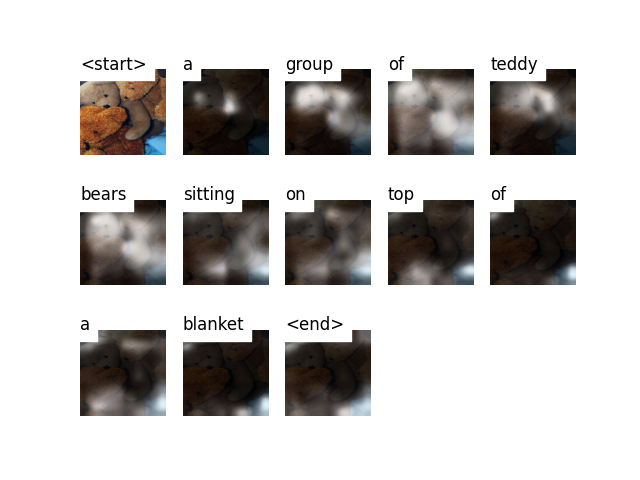
\includegraphics[width=0.9\textwidth]{figures/caption_teddy_normal.png} % first figure itself
    \caption{Prediction by Show Attend and Tell on a clean image. \newline Top left picture is the input image. The highlighted areas in white are the visualization of the attention per predicted word.}
    \label{sat_example}
\end{figure*}

Machine learning models can be very susceptible to noise where small changes to the input can lead to radically different outcomes. As shown by \citeauthor{goodfellow2015explaining} adding a specific (small) noise layer to an image can alter a correct prediction to a very confident wrong prediction. As can be seen in figure \ref{adv_gibbon}. Because the generation of the adversarial examples is not that computational expansive, they can be generated during training making the model more robust. It is also shown that these adversarial examples act as regularizes during training. Reducing the change of overfitting. \citeauthor{Kurakin} expands on generating adversarial examples showing that one can also steer the model towards a specific classification.

\begin{figure*}[h]
    \centering
    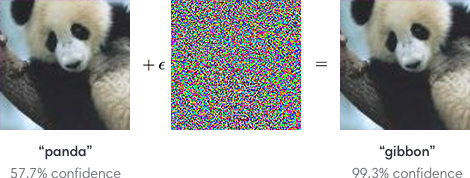
\includegraphics[width=0.9\textwidth]{figures/adversarial_img_1.png}
    \caption{Adversarial noise example from \protect\cite{goodfellow2015explaining}. Where $\epsilon=0.07$.}
    \label{adv_gibbon}
\end{figure*}

Combining these previous findings, S.A.T. can be used to find adversarial examples for image captioning models. These adversarial images can then be used to either improve current datasets by providing hard samples, or in a more malicious way. The latter being especially true when one can specify the output sentence for which an adversarial sample should be created.
Analyzing the successful and failed adversarial samples can also give a better insight in the strengths and weaknesses of S.A.T. Furthermore, it exposes bias present in the datasets.

\subsection*{Research Questions}
This research investigates the susceptibility of S.A.T. against adversarial samples that are visually close but generate completely different descriptions as output.
\begin{itemize}
    \item Is S.A.T. susceptible to adversarial attacks using noise?
    \item Can the noise be crafted in such a way that it can steer the output.
\end{itemize}
